\documentclass[a4paper,12pt,oneside]{book}
\usepackage[utf8]{inputenc}
\usepackage{amssymb}
\usepackage{amsmath}
\usepackage{graphicx}
\graphicspath{ {images/} }
\usepackage{times}
\usepackage{geometry}
\usepackage{setspace}
\usepackage{tocloft}
\usepackage{tabu}
\usepackage{fancyhdr}
\usepackage{tabularx}
\usepackage{caption}

%Defining some new commands for some repeated text.
%Modify your name and other details in this section.
\newcommand{\theauthor}{Tushar Gautam}
\newcommand{\therollno}{114113089}
\newcommand{\thedegree}{B.Tech}
\newcommand{\thedegreelong}{Bachelor of Technology}
\newcommand{\thetitle}{Intelligent estimation of heating and cooling
load requirements of buildings}
\newcommand{\theguide}{Dr.K.Panneerselvam}
\newcommand{\thehod}{Dr.M.Duraiselvam}
\newcommand{\thedepartment}{Production Engineering}
\newcommand{\theyear}{2017}
\newcommand{\theacadyear}{2016-2017}
\newcommand{\themonth}{April}

%Adjusting the caption settings
\captionsetup[figure]{labelfont=bf, textfont=bf}
\captionsetup[table]{labelfont=bf, textfont=bf, position=top}

%Set paragraph indentation to zero
\setlength\parindent{0pt}
%Set paragraph spacing
\setlength{\parskip}{12pt}

%Set the paper size and the margins
\geometry{a4paper, tmargin=1in, rmargin=1in, bmargin=1in, lmargin=1.5in}
\usepackage{titlesec}
\usepackage[hidelinks]{hyperref}

%Format the chapter headings to be 14pt, centered and Uppercase
\titleformat{\chapter}[display]
  {\large\bfseries\centering}
  {\MakeUppercase\chaptertitlename\ \thechapter}{7pt}{\large\MakeUppercase}

%Format the section headings to be uppercase and 12pt
\titleformat{\section}[hang]
  {\MakeUppercase\normalfont\bfseries}
  {\thesection}{12pt}{\MakeUppercase}

%Format the subsections to be 12pt
\titleformat{\subsection}[hang]
  {\MakeUppercase\normalfont\bfseries}
  {\thesubsection}{12pt}{}

%Set the spacing between the chapter headings and the margins
\titlespacing*{\chapter}{0pt}{0pt}{24pt}
\titlespacing*{\section}{0pt}{0pt}{0pt}
\titlespacing*{\subsection}{0pt}{0pt}{0pt}
%Add dots to the table of contents for chapters
\renewcommand{\cftchapleader}{\cftdotfill{\cftdotsep}} % for chapters
%Set the spacings before and after the titles for the TOC, LOF and LOT
\setlength{\cftbeforetoctitleskip}{0.43in}
\setlength{\cftaftertoctitleskip}{21pt}
\setlength{\cftbeforelottitleskip}{0.43in}
\setlength{\cftafterlottitleskip}{21pt}
\setlength{\cftbeforeloftitleskip}{0.43in}
\setlength{\cftafterloftitleskip}{21pt}
%Set the fontsize and formatting for the TOC, LOF and LOT 
\renewcommand\contentsname{\centerline{\fontsize{16pt}{16pt}\selectfont TABLE OF CONTENTS}}
\renewcommand\listfigurename{\centerline{\fontsize{16pt}{16pt}\selectfont LIST OF FIGURES}}
\renewcommand\listtablename{\centerline{\fontsize{16pt}{16pt}\selectfont LIST OF TABLES}}
%Setting page numbers to bottom center
\pagestyle{fancy}
\cfoot{\thepage}
\rhead{}
\lhead{}
\renewcommand{\headrulewidth}{0pt}
\renewcommand{\footrulewidth}{0pt}
%Setting bibliography title format
\renewcommand{\bibname}{\fontsize{16pt}{24pt}\selectfont References \hfill}


\begin{document}
%Adding all the stuff that should be numbered with roman numerals
\frontmatter
\addtocontents{toc}{\textbf{Title}\hfill\textbf{Page No.}\par}
\addtocontents{toc}{\vspace{-0.3cm}}
\begin{titlepage}
\begin{center}
\fontsize{18pt}{1cm}\selectfont \textbf{\MakeUppercase\thetitle}

\vspace*{1.3cm}
\fontsize{14pt}{21pt}\selectfont A thesis submitted in partial fulfillment of the requirements for\\
the award of the degree of

\vspace*{0.4cm}
\fontsize{14pt}{1cm}\selectfont\textbf{\thedegree} 

\vspace*{0.4cm}
\textbf{in\\ \thedepartment}

\vspace*{2.0cm}
By\\
\textbf{\theauthor\ (\therollno)}

\vspace*{2.2cm}

\includegraphics[width=1.25in]{NITT-Logo}


\fontsize{16pt}{16pt}\selectfont \textbf{\MakeUppercase\thedepartment\\NATIONAL INSTITUTE OF TECHNOLOGY\\TIRUCHIRAPPALLI-620015}

\vspace{0.31cm}
\textbf{\MakeUppercase\themonth\ \theyear}
\end{center}
\end{titlepage}

\thispagestyle{plain}
\begin{center}
\textbf{BONAFIDE CERTIFICATE}
\end{center}

\vspace{0.3cm}


\fontsize{12pt}{18pt}\selectfont This is to certify that the project titled \textbf{\MakeUppercase\thetitle} is a bonafide record of the work done by
\vspace{0.1cm}

\begin{center}
\textbf{\theauthor\ (\therollno)}
\end{center}

\vspace{0.1cm}
\noindent
\fontsize{12pt}{18pt}\selectfont in partial fulfillment of the requirements for the award of the degree of \textbf{\thedegreelong} in \textbf{\thedepartment} of the \textbf{NATIONAL INSTITUTE OF TECHNOLOGY, TIRU\-CHIRAPPALLI}, during the year \theacadyear.

\vspace{3cm}

\begin{tabu} to \textwidth { X[c] X[c] X[c] }

 \textbf{\theguide} & \hfill &\textbf{\thehod} \\ 
  Guide & \hfill & Head of the Department

\end{tabu}

\vspace{4cm}
Project Viva-voce held on \rule{5.5cm}{.1pt}

\vspace{4cm}
\textbf{Internal Examiner} \hfill \textbf{External Examiner}

\newpage

\addcontentsline{toc}{chapter}{ABSTRACT}
\addtocontents{toc}{\vspace{-0.3cm}}
\thispagestyle{plain}
\begin{center}
\textbf{\textbf{\fontsize{16pt}{24pt}\selectfont ABSTRACT}}
\end{center}

\vspace{0.3cm}
\fontsize{12pt}{18pt}\selectfont This project studies the effect of various input variables
(relative compactness, surface area, wall area, roof area, overall height, orientation, glazing area, glazing area distribution) on two output variables, namely heating load (HL) and cooling load (CL) of buildings. Reports suggest that building energy consumption has
steadily increased over the past decades worldwide \cite{perez2008pout}, \cite{cai2009ren}, and heating, ventilation and air conditioning
(HVAC), which have a catalytic role in regulating the indoor climate, account for most of the energy use in
the buildings. Therefore, one way to alleviate the ever increasing demand for additional energy supply is to
have more energy-efficient building designs with improved energy conservation properties. When it comes
to efficient building design, the computation of the heating load (HL) and the cooling load (CL) is required to
determine the specifications of the heating and cooling equipment needed to maintain comfortable indoor air
conditions.
Various Machine Learning approach (Regression, ANN etc) is to be studied, implemented,
compared and visualised \cite{Hunter:2007} on the datasets obtained from Machine Learning Repository, Centre for Machine Learning and
Intelligent Systems, UCI. Finally, a model with the best accuracy is proposed.

\textit{Keywords}: Building energy evaluation; Heating load; Cooling load; Regression; ANN

\newpage

\addcontentsline{toc}{chapter}{ACKNOWLEDGEMENTS}
\addtocontents{toc}{\vspace{-0.3cm}}
\thispagestyle{plain}
\begin{center}
\textbf{\textbf{\fontsize{16pt}{24pt}\selectfont ACKNOWLEDGEMENTS}}
\end{center}

I wish to express my sincere thanks to Dr.K.Pannerselvam, for reviewing my work and constant support throughout the project.
I place on record, my sincere thank you to the Dr.M.Duraiselvam and Dr.S.Vinodh for their continuos encouragement to pursue the project in the first place.

I am also grateful to Dr. E.S.Gopi, Assistant Professor, in the Department of Electronics and Communication Engineering. I am extremly thankful and indebted to him for sharing expertise, sincere and valuable guidance and encouragement extended to me. Furthermore, taking a course on Pattern Recognition (EC459) by Dr. E.S. Gopi helped significantly.

I also place on record, my sense of gratitude to one and all, who directly or indirectly, have lent their hand in this venture.

\newpage

\addcontentsline{toc}{chapter}{TABLE OF CONTENTS}
\addtocontents{toc}{\vspace{-0.3cm}}
\tableofcontents
\newpage
\addcontentsline{toc}{chapter}{LIST OF TABLES}
\addtocontents{toc}{\vspace{-0.3cm}}
\listoftables
\newpage
\addcontentsline{toc}{chapter}{LIST OF FIGURES}
\addtocontents{toc}{\vspace{-0.3cm}}
\listoffigures
 
\mainmatter

\chapter{Introduction}
\fontsize{12pt}{18pt}\selectfont
Globally the building sector accounts for more electricity use than any other sector,
42 per cent. No wonder considering that we spend more than 90 per cent of our
time in buildings. With increasing urbanization, higher in developing countries,
the number and size of buildings in urban areas will increase, resulting in an
increased demand for electricity and other forms of energy commonly used in
buildings. Africa’s rate of urbanization of 3.5 per cent per year is the highest in
the world, resulting in more urban areas with bigger populations, as well as the
expansion of existing urban areas. There are currently 40 cities in Africa with
populations of more than a million and it is expected that by 2015 seventy cities
will have populations of one million or more.

In many developing countries there is normally very little margin between existing
power supply and electricity demand. With increasing electricity demand, new
generation needs to be brought in. Although renewable sources of electricity such
as hydro, geothermal or wind provide electricity at a much lower cost, their capital
outlay is large, they are complex and take much longer to implement. Diesel based
generation is usually brought in the short term to meet this demand, which
results in increased cost of electricity.

Investments in energy efficiency in a building can be compared with the cost of
capital investments necessary on the supply side of the energy system to produce
a similar amount of peak capacity or annual energy production. Usually, the
capital costs of efficiency are lower than comparable investments in increased
supply and there are no additional operating costs of efficiency compared to substantial
operating costs for supply-side options. In addition, energy efficiency
investments generally have much shorter lead times than energy supply investments,
a particularly important consideration in countries where the demand for
energy services is growing rapidly.

One consistent quality in the building sector is that it is subject to a high degree
of regulation. Building codes often influence material use and appliance standards
that have a significant effect on energy efficiency. Regulatory regimes, to
the extent that they exist, may therefore provide a pathway to improve efficiency
for both building construction and a variety of building appliances.

Reports \cite{perez2008pout}, \cite{cai2009ren} suggest that heating, ventilation and air conditioning (HVAC), which have a catalytic role in regulating the indoor climate, account for most of the energy use in the buildings. Therefore, one way to alleviate the ever increasing demand for additional energy supply is to have more energy-efficient building designs with improved energy conservation properties. When it comes to efficient building design, the computation of the heating load (HL) and the cooling load (CL) is required to determine the specifications of the heating and cooling equipment needed to maintain comfortable indoor air conditions.

\section {Simulation tools approach}
Building energy simulation tools are currently widely used to analyze or forecast building energy consumption in order to facilitate the design and operation of energy efficient buildings. Simulation tools are used extensively across diverse disciplines because they enable experimentation with parameters that would otherwise be infeasible, or at least very difficult to control in practice \cite{97d2aa88078644a3ab2ef0ca5fd99212}

\section{Machine learning approach}
Using advanced dedicated building energy simulation software may provide reliable solutions to estimate the impact of building design alternatives; however this process can be very time-consuming and requires user expertise in a particular program. Moreover, the accuracy of the estimated results may vary across different building simulation software. Hence, in practice many researchers rely on machine learning tools to study the effect of various building parameters (e.g. compactness) on some variables of interest (e.g. energy) because this is easier and faster if a database of the required ranges of variables is available. Using statistical and machine learning concepts has the distinct advantage that distilled expertise from other disciplines is brought in the EPB domain, and by using these techniques it is extremely fast to obtain answers by varying some building design parameters once a model has been adequately trained. Moreover, statisticalanalysis can enhance our understanding offering quantitative expressions of the factors that affect the quantity (or quantities) of interest that the building designer or architect may wish to focus on.

In this report, various suitable machine learning models (linear and non-linear) have been explored to predict HL and CL.


\chapter{Review of Literature}
\fontsize{12pt}{18pt}\selectfont
Lorem ipsum dolor sit amet, consectetur adipiscing elit. Vivamus at pulvinar nisi. Phasellus hendrerit, diam placerat interdum iaculis, mauris justo cursus risus, in viverra purus eros at ligula. Ut metus justo, consequat a tristique posuere, laoreet nec nibh. Etiam et scelerisque mauris. Phasellus vel massa magna. Ut non neque id tortor pharetra bibendum vitae sit amet nisi. Duis nec quam quam, sed euismod justo. Pellentesque eu tellus vitae ante tempus malesuada. Nunc accumsan, quam in congue consequat, lectus lectus dapibus erat, id aliquet urna neque at massa. Nulla facilisi. Morbi ullamcorper eleifend posuere. Donec libero leo, faucibus nec bibendum at, mattis et urna. Proin consectetur, nunc ut imperdiet lobortis, magna neque tincidunt lectus, id iaculis nisi justo id nibh. Pellentesque vel sem in erat vulputate faucibus molestie ut lorem\cite{perez2008pout}.

\begin{figure}
    \centering
    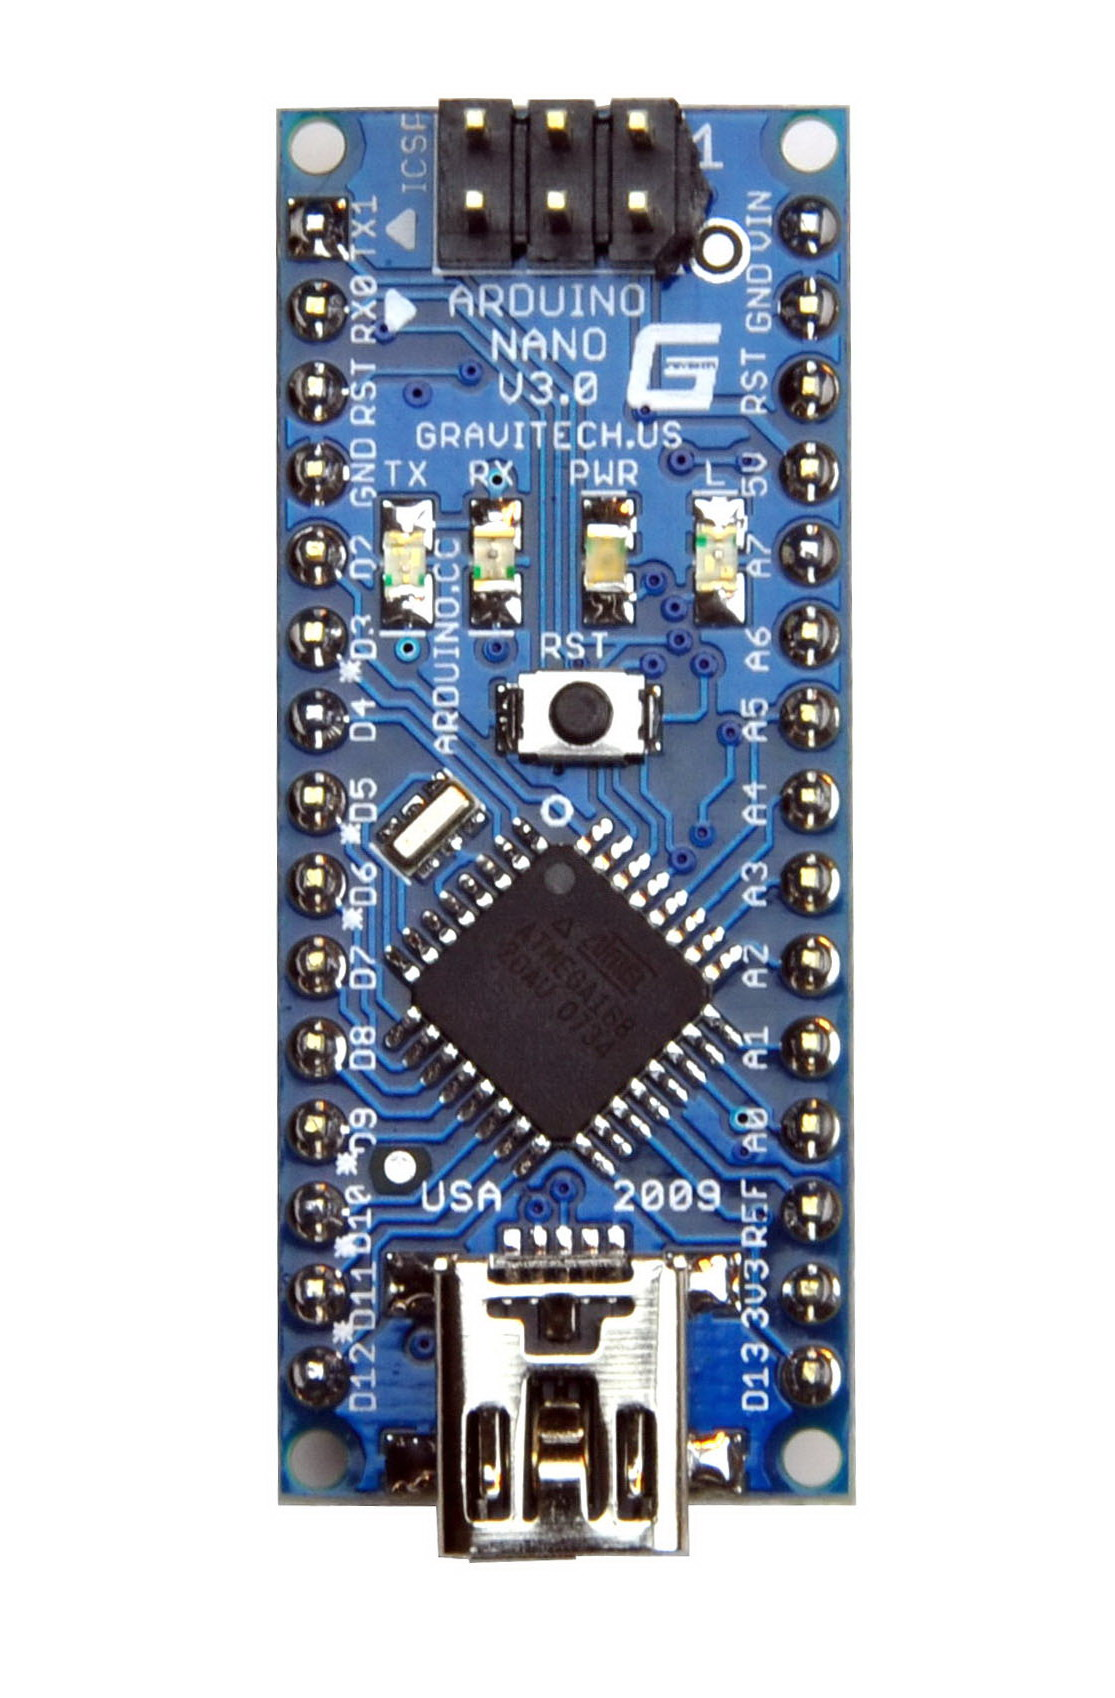
\includegraphics[width=\textwidth]{nano}
    \caption{This is Arduino Nano}
    \label{fig:nano2}
\end{figure}

\section{A Section}

Quisque tristique urna in lorem laoreet at laoreet quam congue. Donec dolor turpis, blandit non imperdiet aliquet, blandit et felis. In lorem nisi, pretium sit amet vestibulum sed, tempus et sem. Proin non ante turpis. Nulla imperdiet fringilla convallis. Vivamus vel bibendum nisl. Pellentesque justo lectus, molestie vel luctus sed, lobortis in libero. Nulla facilisi. Aliquam erat volutpat. Suspendisse vitae nunc nunc. Sed aliquet est suscipit sapien rhoncus non adipiscing nibh consequat. Aliquam metus urna, faucibus eu vulputate non, luctus eu justo \cite{perez2008pout}.

\subsection{A Subsection}

Donec urna leo, vulputate vitae porta eu, vehicula blandit libero. Phasellus eget massa et leo condimentum mollis. Nullam molestie, justo at pellentesque vulputate, sapien velit ornare diam, nec gravida lacus augue non diam. Integer mattis lacus id libero ultrices sit amet mollis neque molestie. Integer ut leo eget mi volutpat congue. Vivamus sodales, turpis id venenatis placerat, tellus purus adipiscing magna, eu aliquam nibh dolor id nibh. Pellentesque habitant morbi tristique senectus et netus et malesuada fames ac turpis egestas. Sed cursus convallis quam nec vehicula. Sed vulputate neque eget odio fringilla ac sodales urna feugiat.

\subsection{B Sub-Section}

Table \ref{table:1} is really awesome and I like it.

The table \ref{table:1} is an example of referenced \LaTeX elements.
 
\begin{table}[h!]
\centering
\begin{tabular}{||c c c c||} 
 \hline
 Col1 & Col2 & Col2 & Col3 \\ [0.5ex] 
 \hline\hline
 1 & 6 & 87837 & 787 \\ 
 2 & 7 & 78 & 5415 \\
 3 & 545 & 778 & 7507 \\
 4 & 545 & 18744 & 7560 \\
 5 & 88 & 788 & 6344 \\ [1ex] 
 \hline
\end{tabular}
\caption{Table to test captions and labels}
\label{table:2}
\end{table}

\section{Another Section}

Phasellus nisi quam, volutpat non ullamcorper eget, congue fringilla leo. Cras et erat et nibh placerat commodo id ornare est. Nulla facilisi. Aenean pulvinar scelerisque eros eget interdum. Nunc pulvinar magna ut felis varius in hendrerit dolor accumsan. Nunc pellentesque magna quis magna bibendum non laoreet erat tincidunt. Nulla facilisi.

Duis eget massa sem, gravida interdum ipsum. Nulla nunc nisl, hendrerit sit amet commodo vel, varius id tellus. Lorem ipsum dolor sit amet, consectetur adipiscing elit. Nunc ac dolor est. Suspendisse ultrices tincidunt metus eget accumsan. Nullam facilisis, justo vitae convallis sollicitudin, eros augue malesuada metus, nec sagittis diam nibh ut sapien. Duis blandit lectus vitae lorem aliquam nec euismod nisi volutpat. Vestibulum ornare dictum tortor, at faucibus justo tempor non. Nulla facilisi. Cras non massa nunc, eget euismod purus. Nunc metus ipsum, euismod a consectetur vel, hendrerit nec nunc.

\begin{figure}
    \centering
    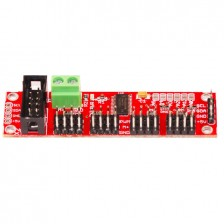
\includegraphics{servo_driver}
    \caption{This is a servo controller.}
    \label{fig:servo_driver2}
\end{figure}

Single equation
\begin{equation}
    e^{i\pi} = -1
\end{equation}

Multiple equations
\begin{align}
\textnormal{State Vector: }& x = \begin{bmatrix}q&\vec{\omega}\end{bmatrix}^T \\
\textnormal{Process Model: }& x_{k+1} = A(x_k, w_k) = \begin{bmatrix}q_kq_wq_{\Delta}\\\omega_{k}\end{bmatrix}\\
\textnormal{Measurement Model: }& z_k = H(x_k, v_k) = \begin{bmatrix}q_kgq_k^* + \vec{v}_{acc}\\\vec{\omega}_k + \vec{v}_{rot}\end{bmatrix}
\end{align}

This is an example of how you can reference an image. This sentence is referring to the Figure \ref{fig:tree}

\begin{figure}
    \centering
    %includegraphics[width=\textwidth]{KinematicTree}
    \caption{This is some awesome thing.}
    \label{fig:tree2}
\end{figure}


\chapter{Data exploration}
\fontsize{12pt}{18pt}\selectfont
\section{Dataset description}
  The dataset contains eight attributes (or features, denoted by X1...X8) and two responses (or outcomes, denoted by y1 and y2).
  \begin{table}[h!]
  \parbox{.45\linewidth}{
          \centering
          \caption{Features}
          \label{tab:table1}
          \begin{tabular}{|c|}
            Relative compactness (X1)\\
            \hline
            Surface area (X2)\\
            \hline
            Wall area (X3)\\
            \hline
            Roof area (X4)\\
            \hline
            Overall height (X5)\\
            \hline
            Orientation (X6)\\
            \hline
            Glazing area (X7)\\
            \hline
            Glazing area distribution (X8)\\
            \hline            
          \end{tabular}
  }
  \hfill
  \parbox{.45\linewidth}{
          \centering
          \caption{Responses}
          \label{tab:table2}
          \begin{tabular}{|c|}
            Cooling load (y1)\\
            \hline
            Heating load (y2)\\
            \hline           
          \end{tabular}
  }
  \end{table}
  
  \subsection{Mapping}
    The aim is to use the eight features to predict each of the two responses.
    \begin{equation}
         f\colon \begin{array}{>{\displaystyle}r @{} >{{}}c<{{}} @{} >{\displaystyle}l} 
          X &\rightarrow& Y \\ 
          X &\mapsto& f(X) 
         \end{array}
    \end{equation}
        
  \section{Probability density}
  The first step in most data analysis applications is the exploration of the statistical properties of the variables. This is typically achieved   by plotting the probability densities, which succinctly summarize each variable for visualization. One way to obtain an empirical non-parametric density estimate is by using histograms. Although histograms are considered crude for most advanced statistical applications, they have the great advantage of making no prior assumptions regarding the distribution of the examined variable and are very simple to compute. \textit{Often, this preliminary step can reveal whether the variable follows a Gaussian (normal) distribution, which is characterized by a unimodal peak in the middle of the variable’s possible range of values, is completely symmetric}, and is particularly useful because a large number of mathematical functions are applicable \cite{bishop}.

\subsection{Histograms}

\begin{figure}[h!]
    \centering
    \begin{minipage}{0.45\textwidth}
      \centering
      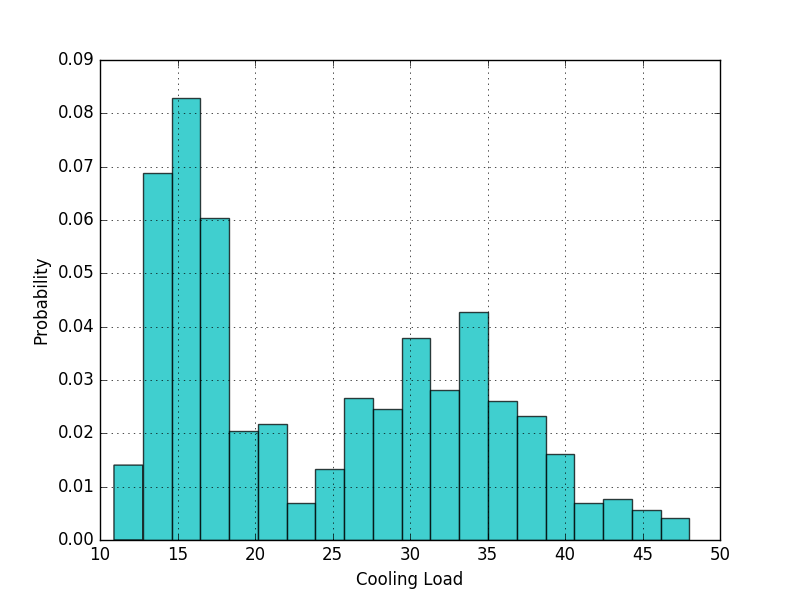
\includegraphics[width=1\textwidth]{hist_cl}
      \caption{Cooling load (y1)}
      \label{fig:hist_cl}
    \end{minipage}\hfill
    \begin{minipage}{0.45\textwidth}
      \centering
      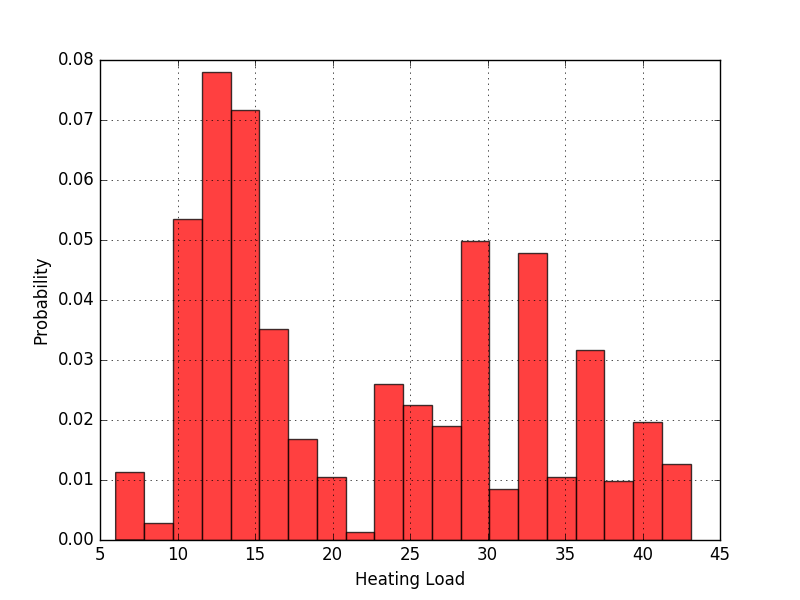
\includegraphics[width=1\textwidth]{hist_hl}
      \caption{Heating load (y2)}
      \label{fig:hist_hl}
    \end{minipage}
\end{figure}
\begin{figure}[h!]
    \centering
    \begin{minipage}{0.45\textwidth}
      \centering
      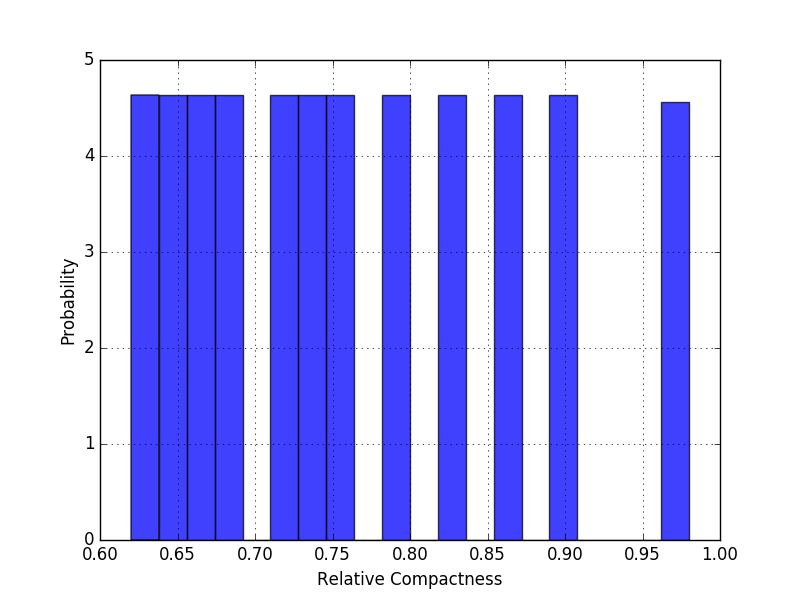
\includegraphics[width=1\textwidth]{hist_rc}
      \caption{Rel. compactness (X1)}
      \label{fig:hist_rc}
    \end{minipage}\hfill
    \begin{minipage}{0.45\textwidth}
      \centering
      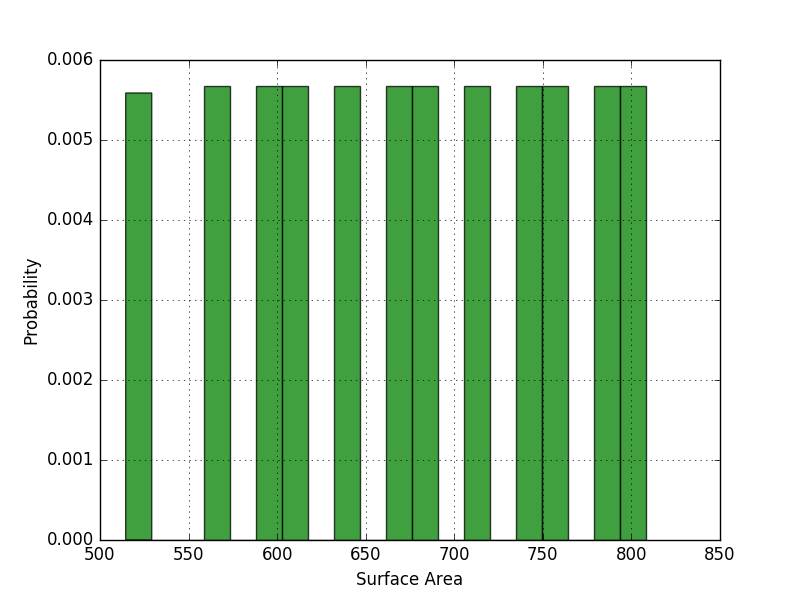
\includegraphics[width=1\textwidth]{hist_sa}
      \caption{Surface area (X2)}
      \label{fig:hist_sa}
    \end{minipage}
\end{figure}
\begin{figure}[h!]
    \centering
    \begin{minipage}{0.45\textwidth}
      \centering
      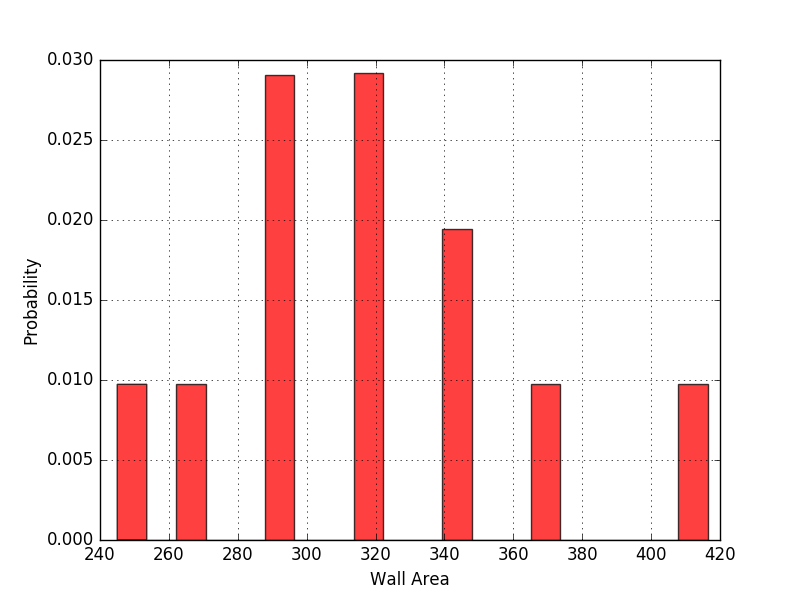
\includegraphics[width=1\textwidth]{hist_wa}
      \caption{Wall area (X3)}
      \label{fig:hist_wa}
    \end{minipage}\hfill
    \begin{minipage}{0.45\textwidth}
      \centering
      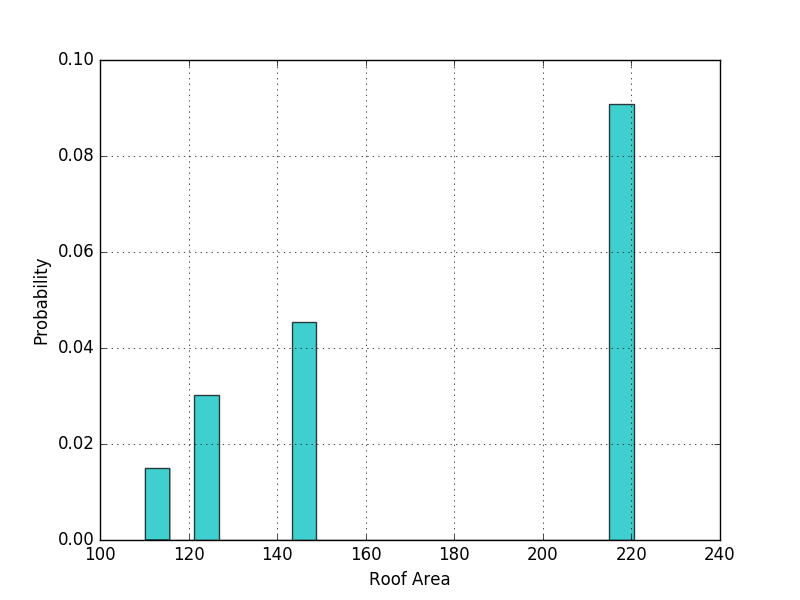
\includegraphics[width=1\textwidth]{hist_ra}
      \caption{Roof area (X4)}
      \label{fig:hist_ra}
    \end{minipage}
\end{figure}
\begin{figure}[h!]
    \centering
    \begin{minipage}{0.45\textwidth}
      \centering
      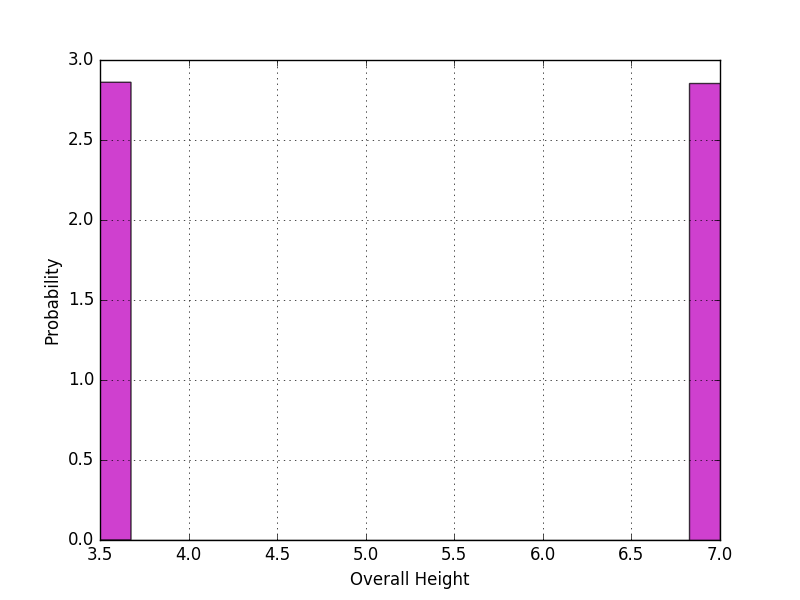
\includegraphics[width=1\textwidth]{hist_oh}
      \caption{Overall height (X5)}
      \label{fig:hist_oh}
    \end{minipage}\hfill
    \begin{minipage}{0.45\textwidth}
      \centering
      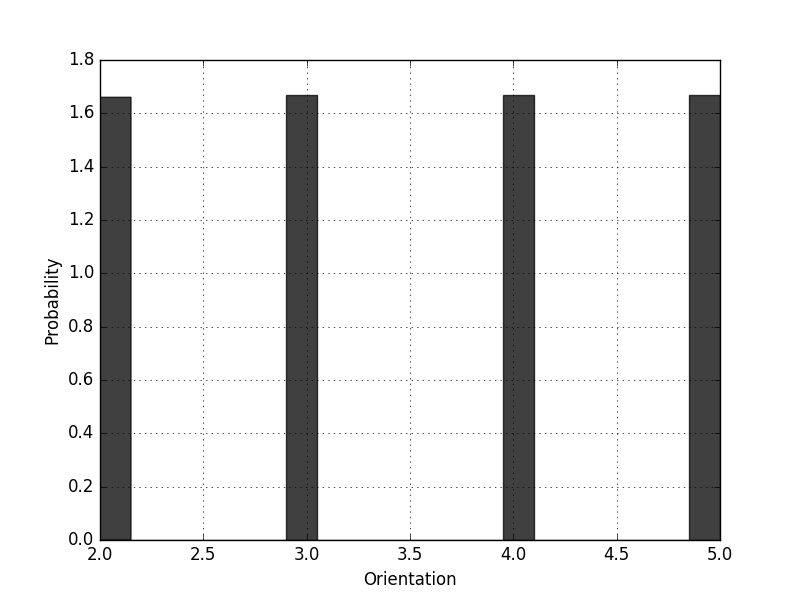
\includegraphics[width=1\textwidth]{hist_or}
      \caption{Orientation (X6)}
      \label{fig:hist_or}
    \end{minipage}
\end{figure}
\begin{figure}[h!]
    \centering
    \begin{minipage}{0.45\textwidth}
      \centering
      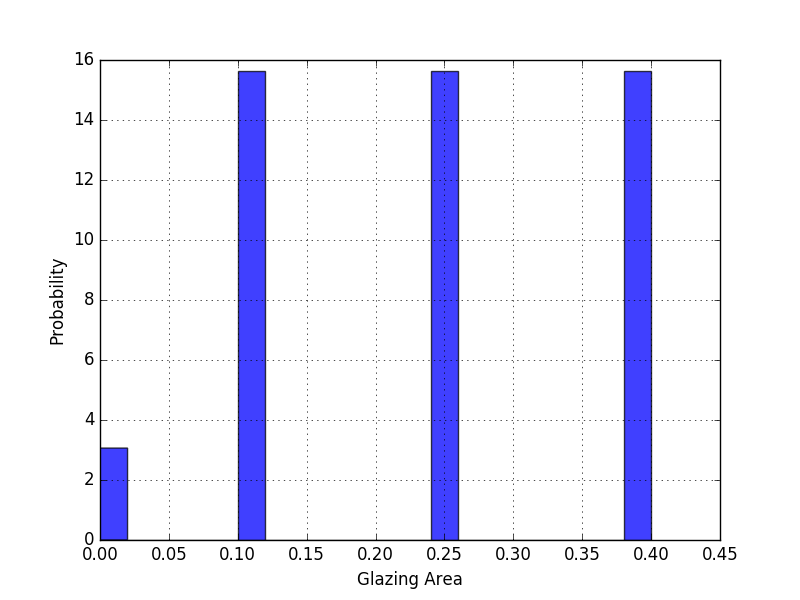
\includegraphics[width=1\textwidth]{hist_ga}
      \caption{Glazing area (X7)}
      \label{fig:hist_ga}
    \end{minipage}\hfill
    \begin{minipage}{0.45\textwidth}
      \centering
      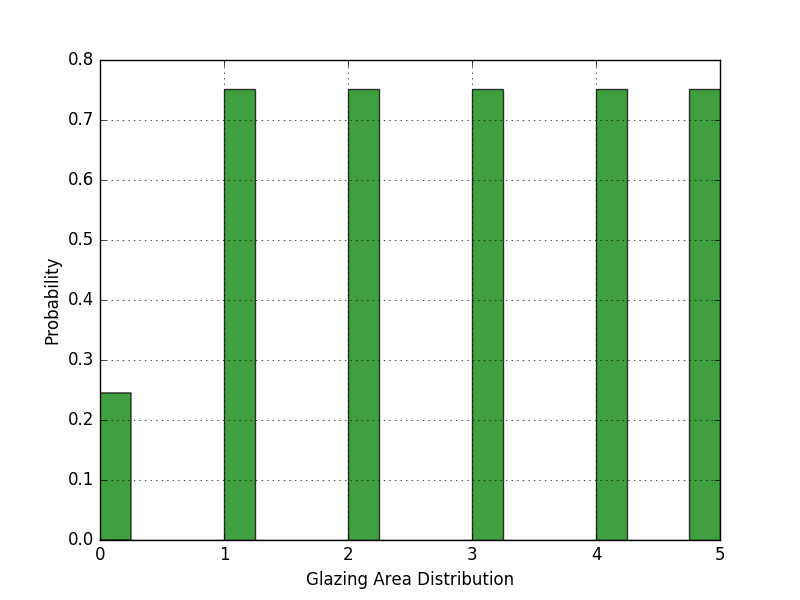
\includegraphics[width=1\textwidth]{hist_gad}
      \caption{Glazing area distribution (X8)}
      \label{fig:hist_gad}
    \end{minipage}
\end{figure}
\newpage
\subsection{Conclusion}
We observe that there is no unimodal peak in the middle or the symmetry. Hence, the data is non-Gaussian.

\section{Correlation}
  \subsection{Scatter plot}
    Scatter plots are similar to line graphs in that they use horizontal and vertical axes to plot data points. However, they have a very specific purpose. Scatter plots show how much one variable is affected by another. The relationship between two variables is called their correlation. For simplicity, scatter plots often use normalized data (i.e. all the variables are normalized to lie between 0 and 1) to facilitate comparison between measures that possibly span orders of magnitude different ranges of values.
Correlation plot between different features and between features and responses have been shown below:    
    \begin{figure}
      \centering
      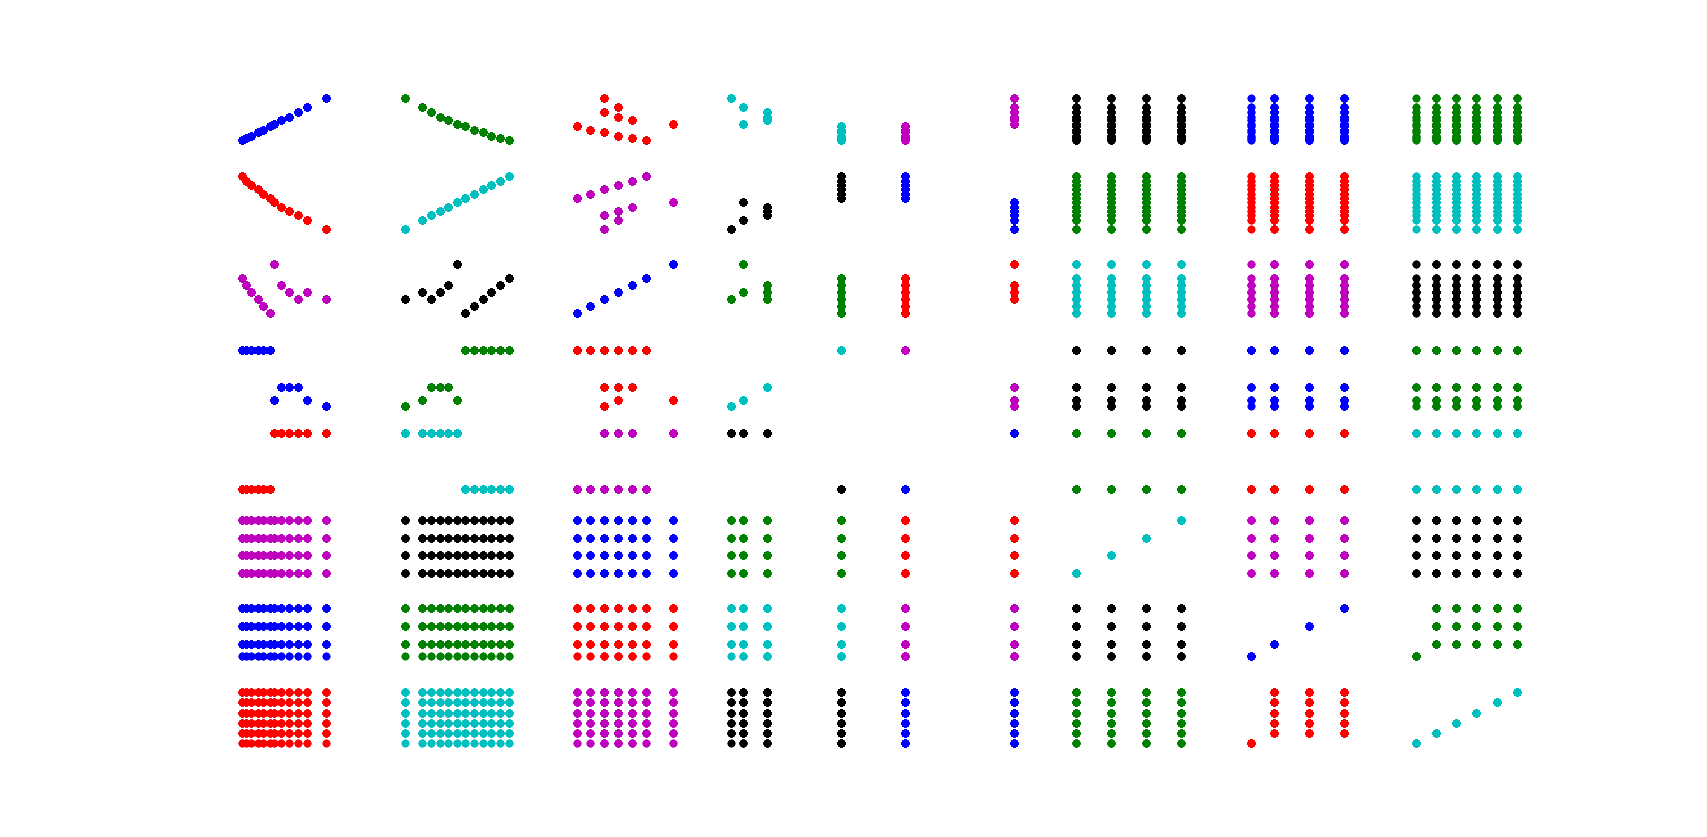
\includegraphics[width=1\textwidth]{scatter_xx}
      \caption{Scatter plot grid between features (X)}
      \label{fig:scatter_xx}
    \end{figure}
    \begin{figure}
      \centering
      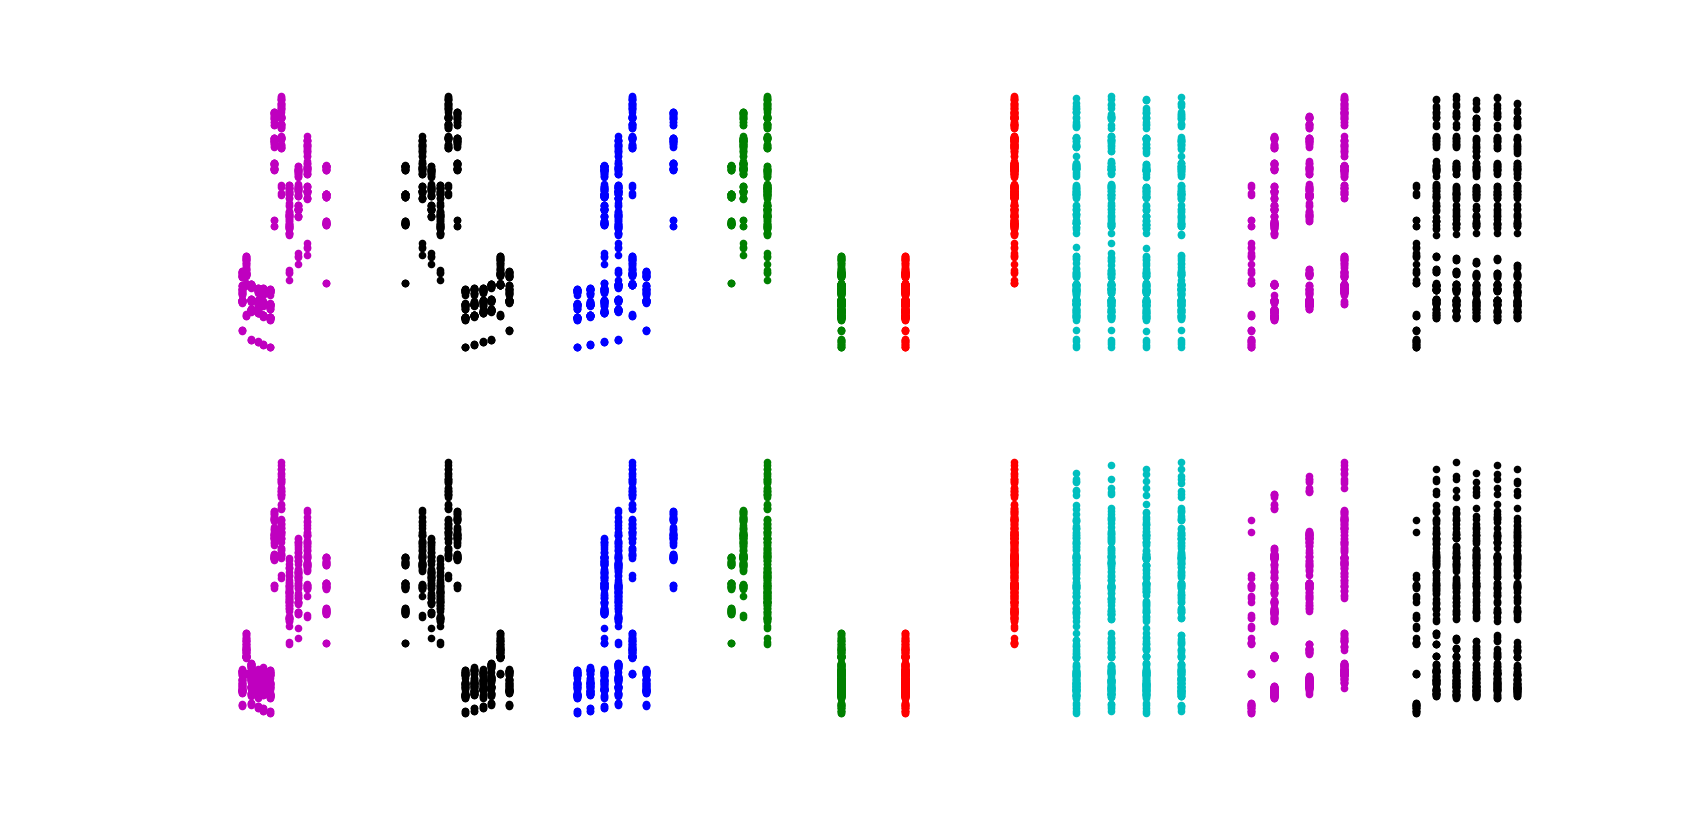
\includegraphics[width=1\textwidth]{scatter_xy}
      \caption{Scatter plot grid between features (X) vs responses (Y)}
      \label{fig:scatter_xy}
    \end{figure}
  \subsection{Spearman rank correlation coefficient}
    As concluded from the histogram plot above, the data is non-Gaussian, so we use the Spearman rank correlation coefficient to obtain a statistical metric regarding the association strength of each input variable with each of the two outputs. The Spearman rank correlation coefficient can characterize general monotonic relationships and lies in the range [-1 1], where negative sign indicates inversely proportional and positive sign indicates proportional rela- tionship, whilst the magnitude denotes how strong this relationship is.
    \begin{figure}[htbp]
      \hspace*{-2.1cm}
      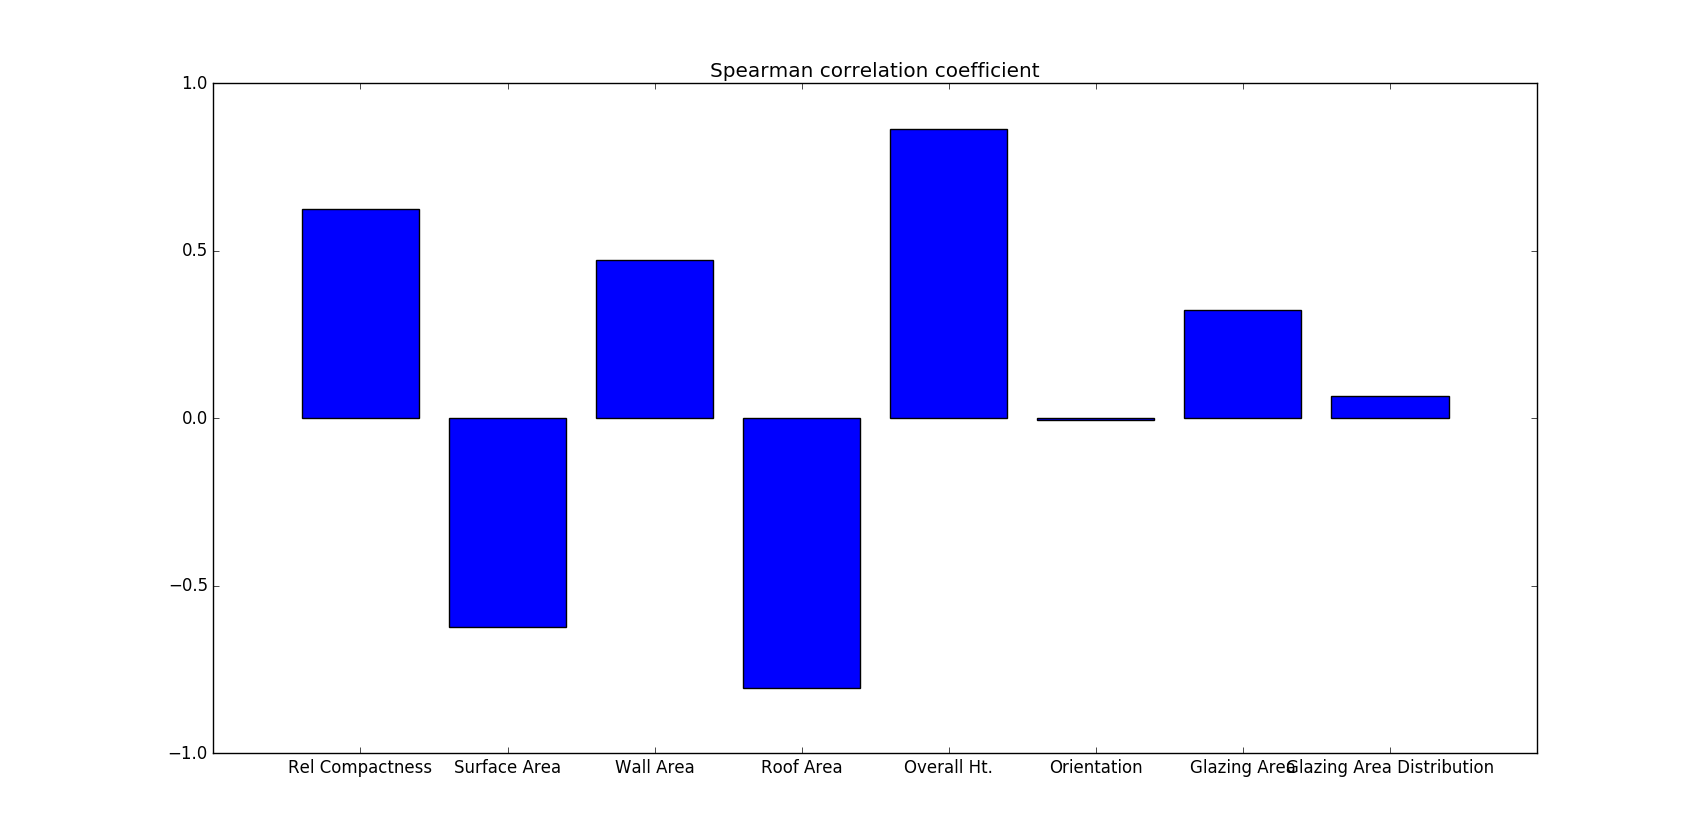
\includegraphics[width=1.3\textwidth]{sp_coeff}
      \caption{Spearman rank correlation coeff. for various features}
      \label{fig:sp_coeff}
    \end{figure}
    \newpage
    \begin{table}[h!]
          \centering
          \caption{Association strength estimated using the Spearman rank correlation coefficient of the eight input variables (X1. . . X8) with heating load (y1).}
          \label{tab:sprcoeffhl}
          \begin{tabular}{c|c}
            Features & Spearman rank correlation coefficient\\
            \hline
            X1 & 0.623 \\
            \hline
            X2 & -0.623 \\
            \hline
            X3 & 0.471 \\
            \hline
            X4 & -0.806 \\
            \hline
            X5 & 0.861 \\
            \hline
            X6 & -0.004 \\
            \hline
            X7 & 0.323 \\
            \hline
            X8 & 0.068 \\
            \hline
          \end{tabular}
    \end{table}
    
    \begin{table}[h!]
          \centering
          \caption{Association strength estimated using the Spearman rank correlation coefficient of the eight input variables (X1. . . X8) with cooling load (y2).}
          \label{tab:sprcoeffcl}
          \begin{tabular}{c|c}
            Features & Spearman rank correlation coefficient\\
            \hline
            X1 & 0.651 \\
            \hline
            X2 & -0.651 \\
            \hline
            X3 & 0.416 \\
            \hline
            X4 & -0.803 \\
            \hline
            X5 & 0.865 \\
            \hline
            X6 & 0.018 \\
            \hline
            X7 & 0.289 \\
            \hline
            X8 & 0.046 \\
            \hline
          \end{tabular}
    \end{table}
    \subsection{Correlation Matrix for features(X)}
          \begin{equation}
            \Corr(X, Y) = \frac{\Cov(X, Y)}{\sigma_{x}\sigma_{y}} = \frac{\E[(X-\mu_{x})(Y-\mu_{y})]}{\sigma_{x}\sigma_{y}}  
          \end{equation}
          \newline
          \begin{equation}
            \left[
              \begin{matrix}
                  1.0 & -1.0 & -0.254 & -0.870 & 0.869 & 0.002 & 0.003 & 0.003\\
-1.0 & 1.0 & 0.254 & 0.870 & -0.869 & -0.002 & -0.004 & -0.003\\
-0.254 & 0.254 & 1.0 & -0.195 & 0.221 & -0.001 & -0.001 & -0.001\\
-0.870 & 0.870 & -0.195 & 1.0 & -0.937 & -0.003 & -0.003 & -0.003\\
0.869 & -0.869 & 0.221 & -0.937 & 1.0 & 0.002 & 0.002 & 0.002\\
0.002 & -0.002 & -0.001 & -0.003 & 0.002 & 1.0 & -0.003 & -0.003\\
0.003 & -0.004 & -0.002 & -0.003 & 0.002 & -0.003 & 1.0 & 0.184\\
0.003 & -0.003 & -0.001 & -0.003 & 0.002 & -0.003 & 0.184 & 1.0
              \end{matrix}
            \right]
    \end{equation}
    \begin{figure}[htbp]
      \hspace*{-6.1cm}
      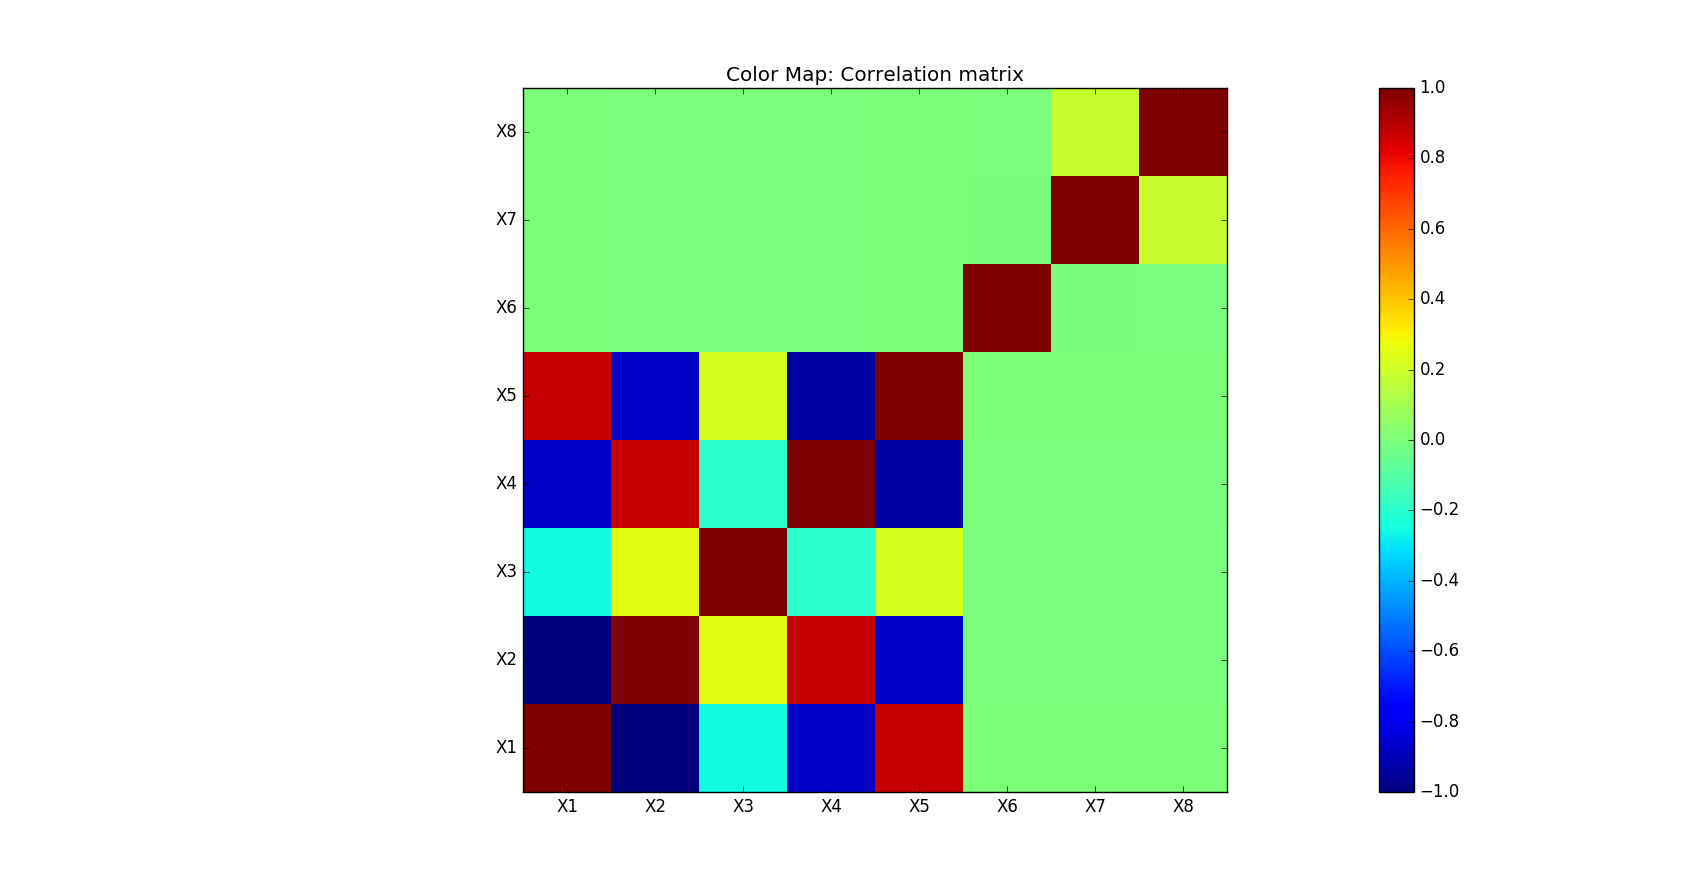
\includegraphics[width=1.7\textwidth]{cov_matrix}
      \caption{Correlation matrix shown as Color Map}
      \label{fig:cov_matrix}
    \end{figure}
    \newpage  
  \subsection{Conclusion}
  Figure \ref{fig:hist_rc} presents the empirical probability distributions of all the input and output variables. These distributions demonstrate that none of the variables follows the normal distribution. Figure \ref{fig:scatter_xy} displays the scatter plots for each of the (normalized) input variables with each of the two output variables. These scatter plots and Color Map show that any functional relationship of the input variables and the output variables is not trivial. This suggests that we can reasonably expect that classical learners such as linear regression (linear models) may fail to find an accurate mapping of the input variables to the output variables. Therefore, these plots intuitively justify the need to experiment with complicated learners such as Artificial Neural Networks (non linear models).


\chapter{Machine learning approach}
\fontsize{12pt}{18pt}\selectfont
\section{Linear models}
  


\chapter{Results and Discussions}
\fontsize{12pt}{18pt}\selectfont
Hello


\chapter{Summary and Conclusions}
\fontsize{12pt}{18pt}\selectfont
\section{Model accuracy}
  \subsection{Linear vs Non-linear model}
  \subsubsection{Cross validation}
    One of the main reasons for using cross-validation instead of using the conventional validation (e.g. partitioning the data set into two sets of 70\% for training and 30\% for test) is that there is not enough data available to partition it into separate training and test sets without losing significant modelling or testing capability. In these cases, a fair way to properly estimate model prediction performance is to use cross-validation as a powerful general technique. In summary, cross-validation combines (averages) measures of fit (prediction error) to derive a more accurate estimate of model prediction performance.
  \subsubsection{Accuracy plot}
  \begin{figure}[h!]
      \centering
      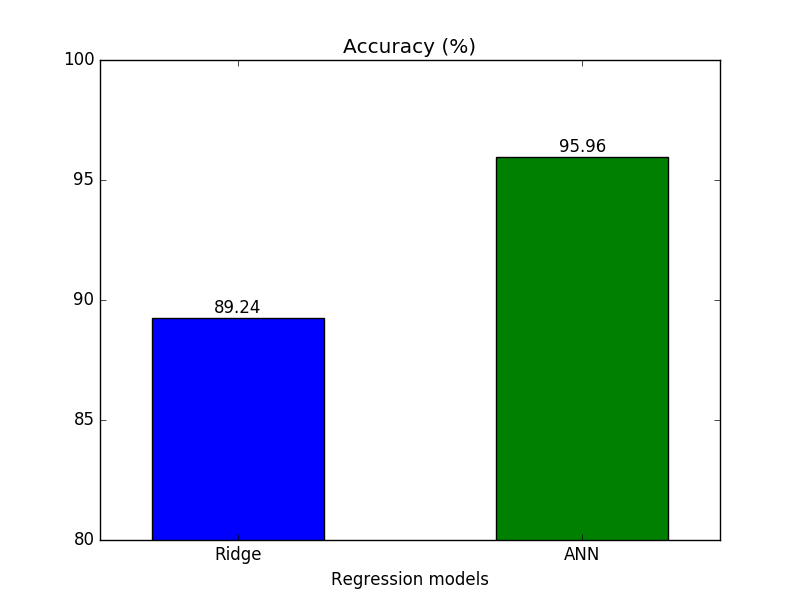
\includegraphics[width=0.7\linewidth]{accuracy.png}
      \caption{Models accuracy : Linear (Ridge) vs Non-linear (ANN)}
      \label{fig:accuracy}                    
  \end{figure}
  \newpage
  As observed before, the data has non-linear relationship with responses. The probability distributions demonstrate that none of the variables follows the normal distribution. Furthermore, the scatter plots show that any functional relationship of the input variables and the output variables is not trivial. This suggests that we can reasonably expect that classical learners such as linear regression (linear models) may fail to find an accurate mapping of the input variables to the output variables. Therefore, these insights intuitively show the need for non-linear models. This claim can be justified by comparing the fitting of a linear model (Ridge regression) and non-linear model (ANN) shown below:

  \subsubsection{Ridge}
  \begin{figure}[h!]
      \centering
      \includegraphics[width=0.9\linewidth]{to_ridge_cl}
      \caption{Target CL, Output CL and corresponding error (target-output) plot}
      \label{fig:to_ridge_cl}                    
  \end{figure}
  \begin{figure}[h!]
      \centering
      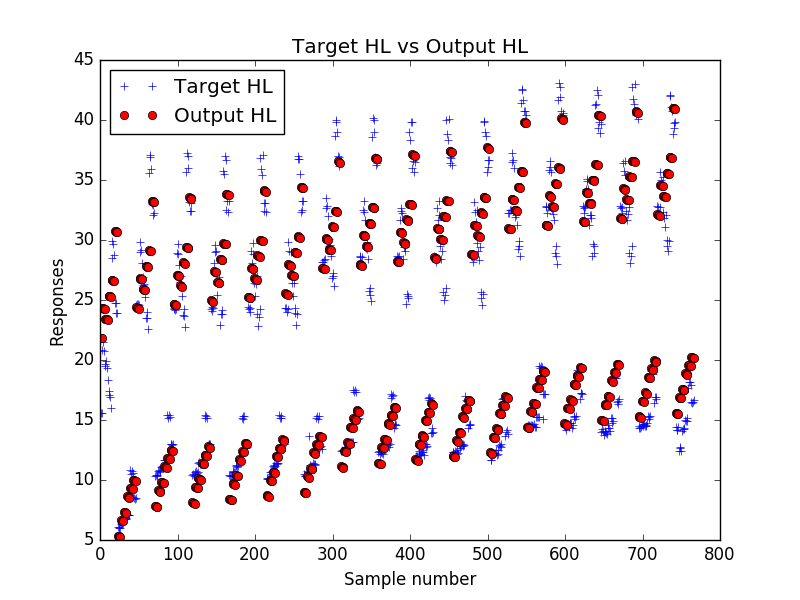
\includegraphics[width=0.9\linewidth]{to_ridge_hl}
      \caption{Target HL, Output HL and corresponding error (target-output) plot}
      \label{fig:to_ridge_hl}                    
  \end{figure}
  \newpage
  \subsubsection{ANN}
  \begin{figure}[h!]
      \centering
      \includegraphics[width=0.9\linewidth]{to_ann_cl}
      \caption{Target CL, Output CL and corresponding error (target-output) plot}
      \label{fig:to_ann_cl}                    
  \end{figure}
  \begin{figure}[h!]
      \centering
      \includegraphics[width=0.9\linewidth]{to_ann_hl}
      \caption{Target HL, Output HL and corresponding error (target-output) plot}
      \label{fig:to_ann_hl}                    
  \end{figure}
  


\bibliography{tushar_refs}{}
\addcontentsline{toc}{chapter}{REFERENCES}
\bibliographystyle{unsrt}
\end{document}
